\section{Numerical Tests}

\subsection{Accuracy Tests}
To compare the accuracy of the IMEX scheme, we applied our PDARSs with RKCB2 [citation] and SSP2332[citation] scheme to some smooth problems in streaming, absorption, ans scattering dominated regimes in one spatial dimension.
All the tests in this subsection were applied with third order accurate spatial discretization, the maximum entropy closure in the low occupancy limit and time step $\dt = 0.1 \times \dx $.
More information and the definition of the absolute error and the relative error can be found in \cite{Chu_2018}.

\subsubsection{Sine Wave Streaming}
This test involves the streaming part only: the collision term is turned off. 
A periodic domain $D$ was applied and the initial condition 
\begin{figure}[h]
  \centering
    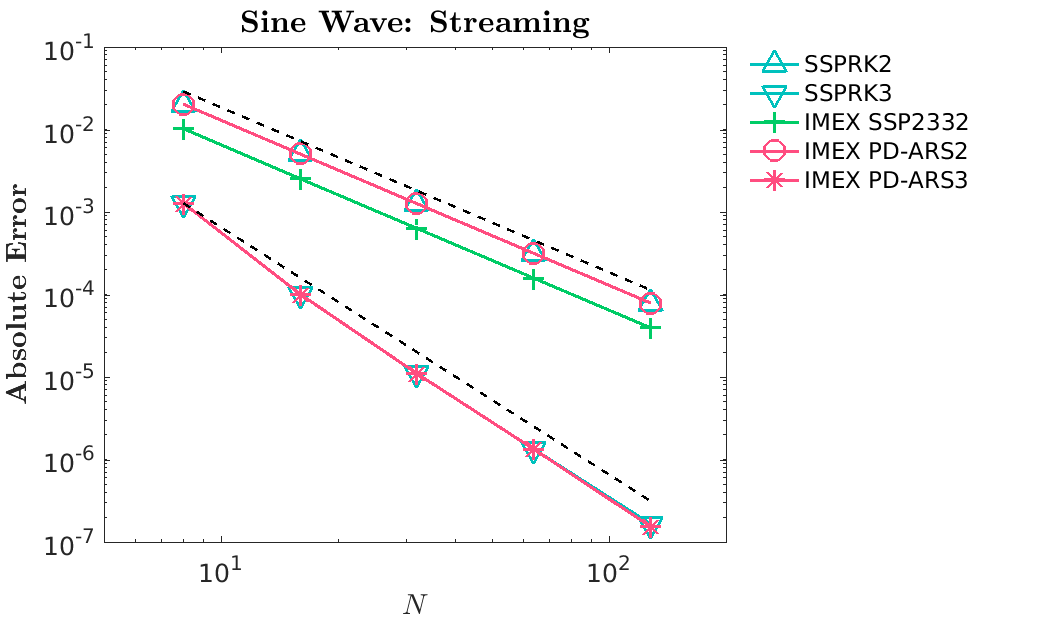
\includegraphics[width=0.6\textwidth]{figures/SineWaveStreaming}
   \caption{Sine Wave Streaming}
\end{figure}

\subsubsection{Sine Wave Damping}
\begin{figure}[h]
  \centering
    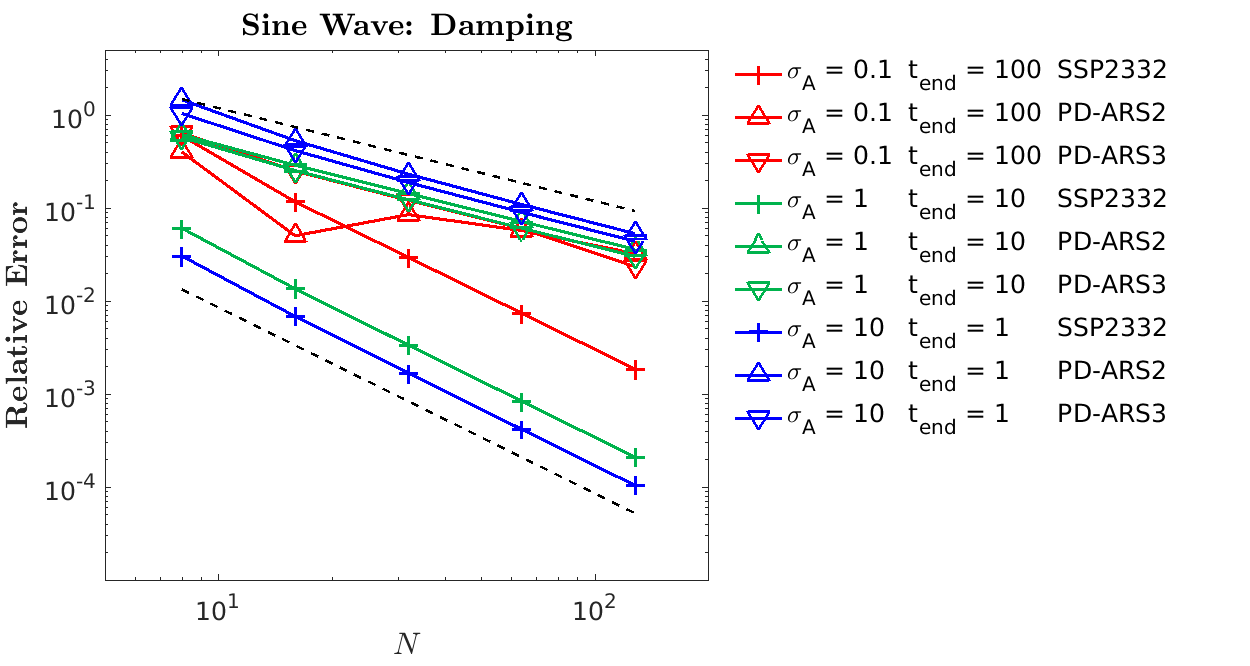
\includegraphics[width=0.7\textwidth]{figures/SineWaveDamping}
   \caption{Sine Wave Damping}
\end{figure}
\subsubsection{Sine Wave Diffusion}
\begin{figure}[h]
  \centering
  \begin{tabular}{cc}
    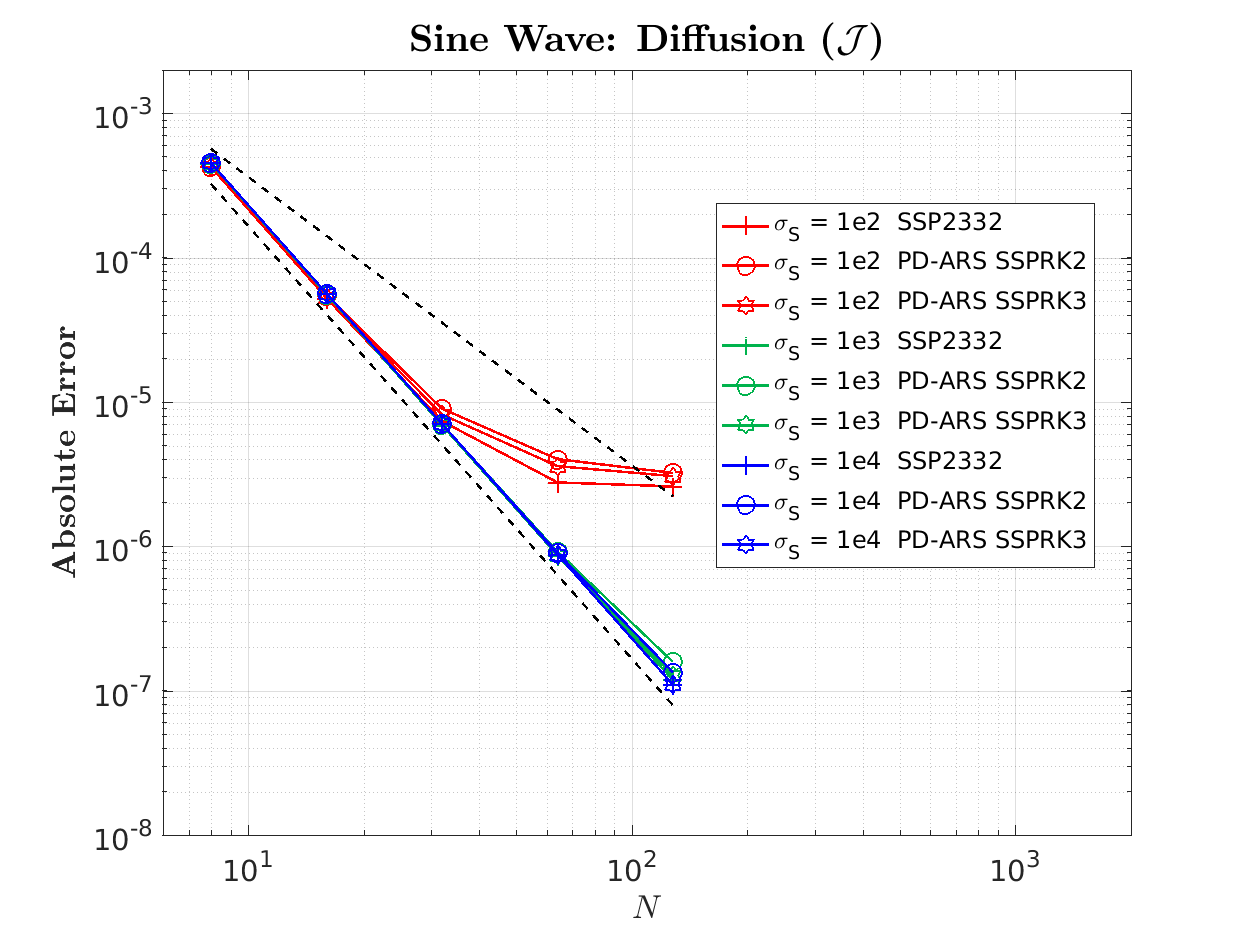
\includegraphics[width=0.5\textwidth]{figures/SineWaveDiffusionJ}
    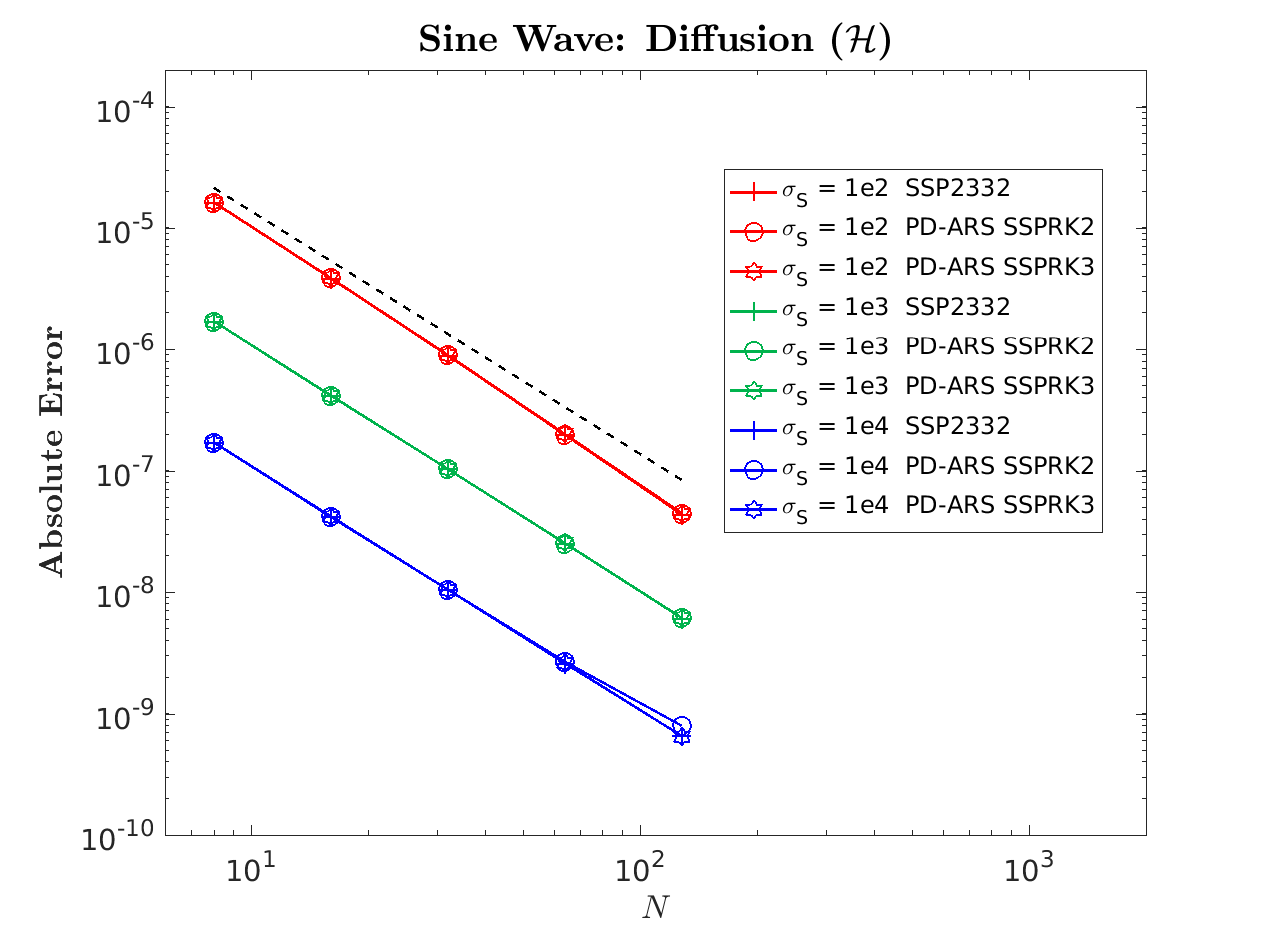
\includegraphics[width=0.5\textwidth]{figures/SineWaveDiffusionH}
  \end{tabular}
   \caption{Sine Wave Diffusion}
\end{figure}

\subsection{Constraint-Preserving Tests}


\subsubsection{Neutrino Stationary State Test}
\begin{figure}[h]
  \centering
  \begin{tabular}{cc}
    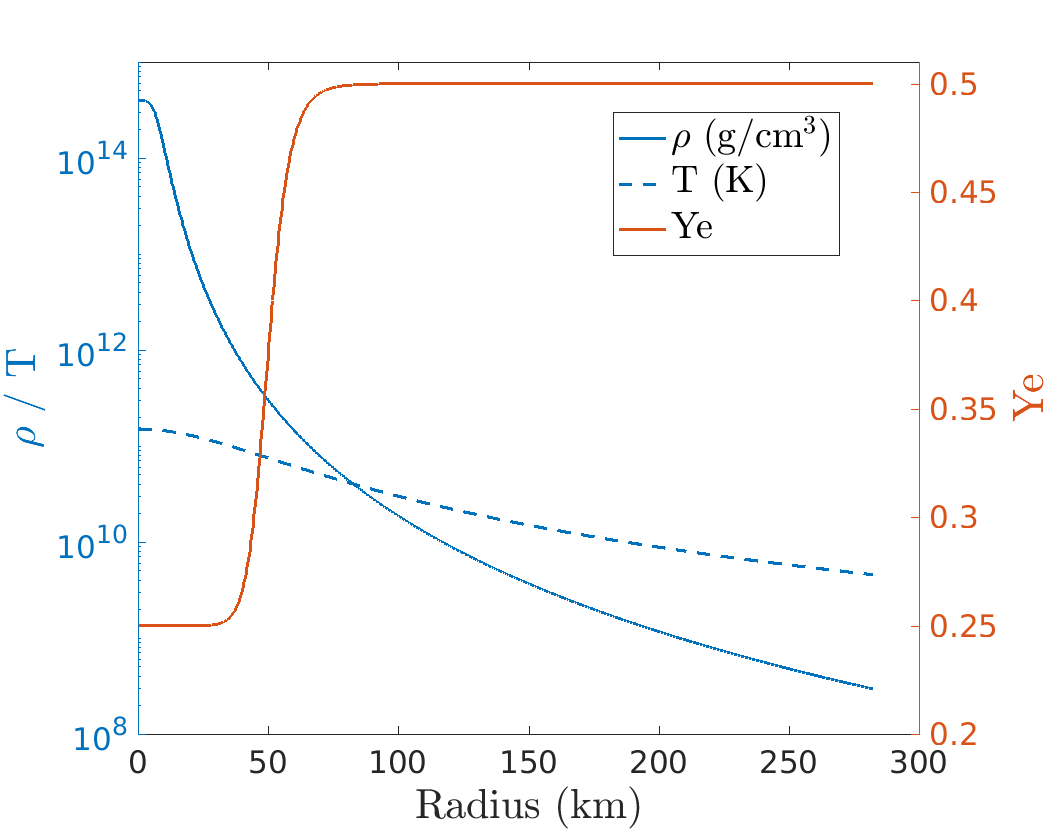
\includegraphics[width=0.4\textwidth]{figures/NStatinaryS_EOS}
    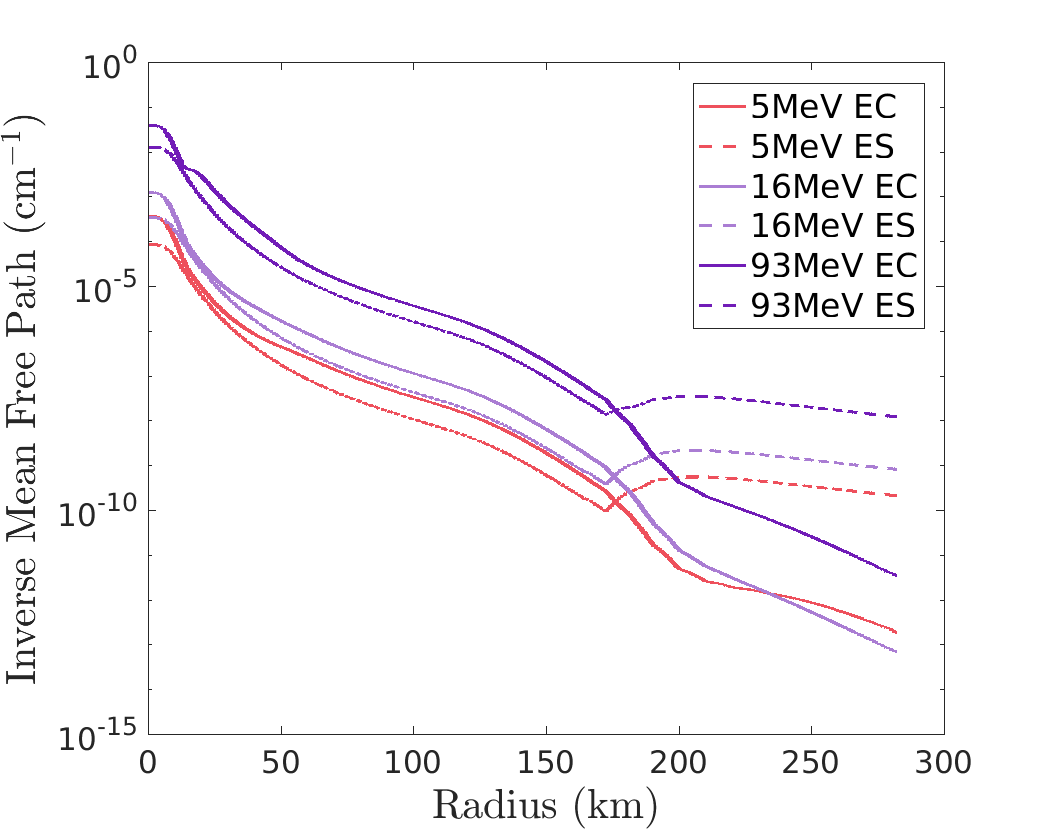
\includegraphics[width=0.55\textwidth]{figures/NSS_Opacities}
  \end{tabular}
   \caption{Neutrino Stationary State Test}
\end{figure}

\begin{figure}[h]
  \centering
  \begin{tabular}{cc}
    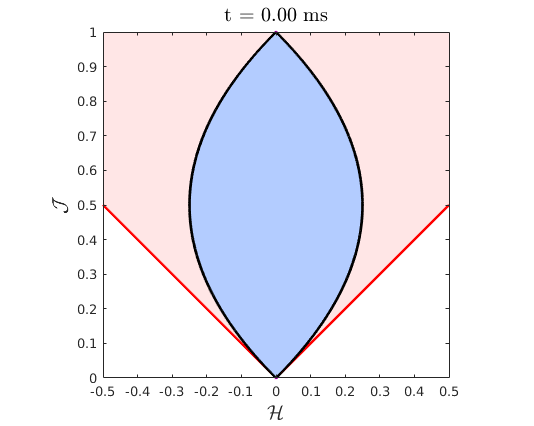
\includegraphics[width=0.45\textwidth]{figures/NSS_0_1}
    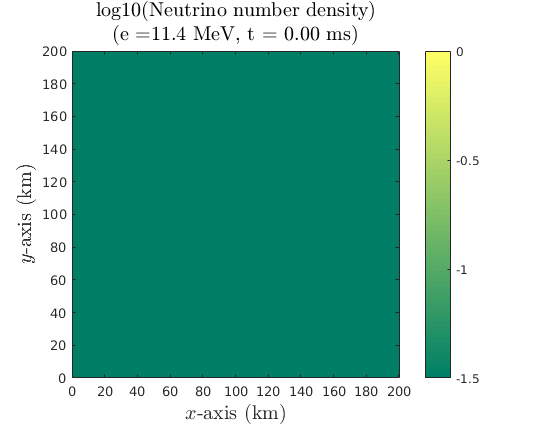
\includegraphics[width=0.45\textwidth]{figures/NSS_0_2} \\
    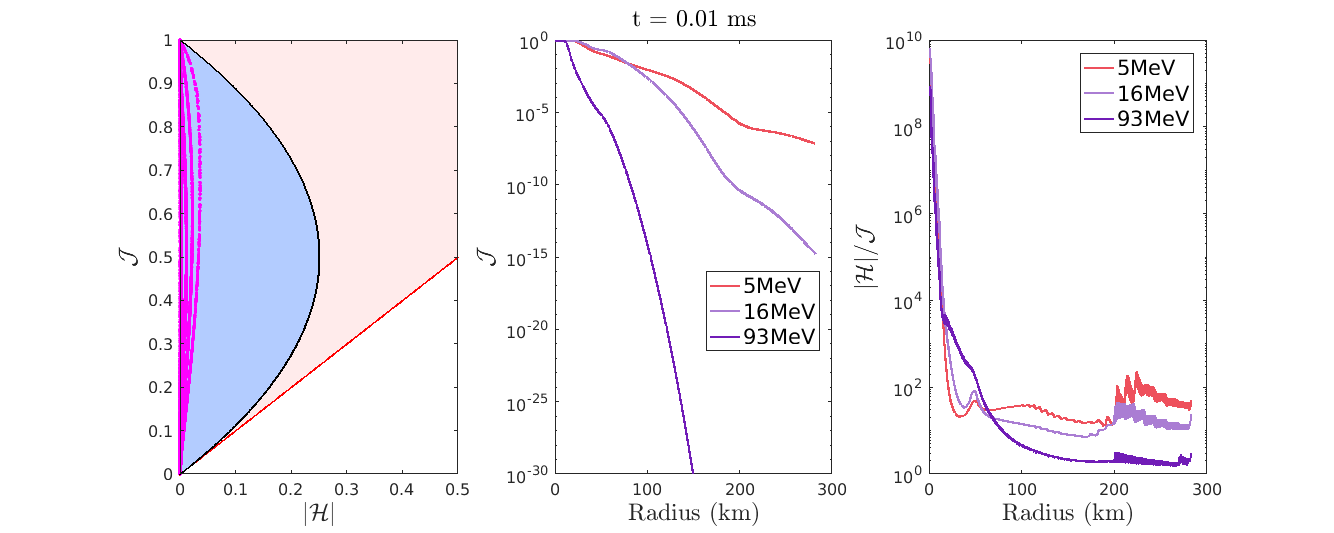
\includegraphics[width=0.45\textwidth]{figures/NSS_1_1}
    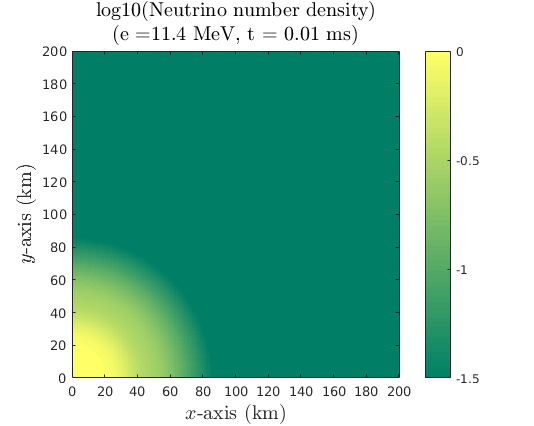
\includegraphics[width=0.45\textwidth]{figures/NSS_1_2} \\
    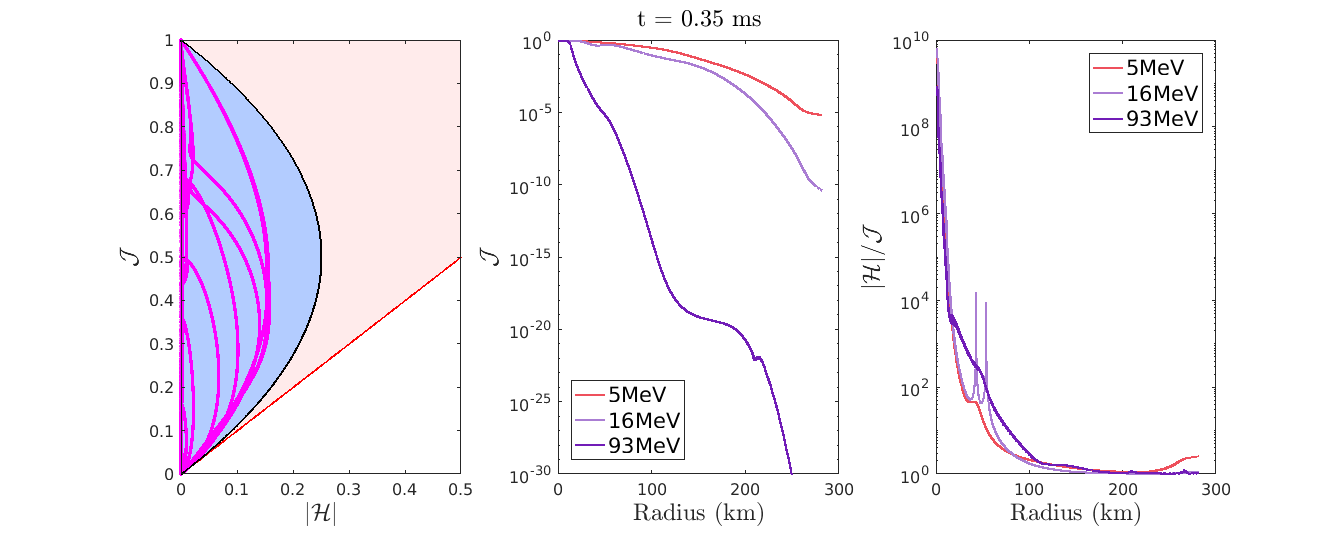
\includegraphics[width=0.45\textwidth]{figures/NSS_3_1}
    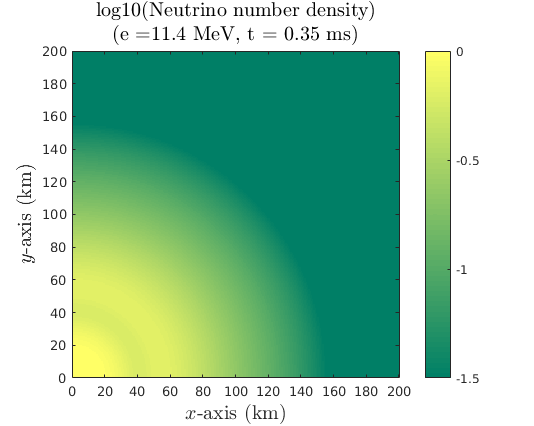
\includegraphics[width=0.45\textwidth]{figures/NSS_3_2} \\
    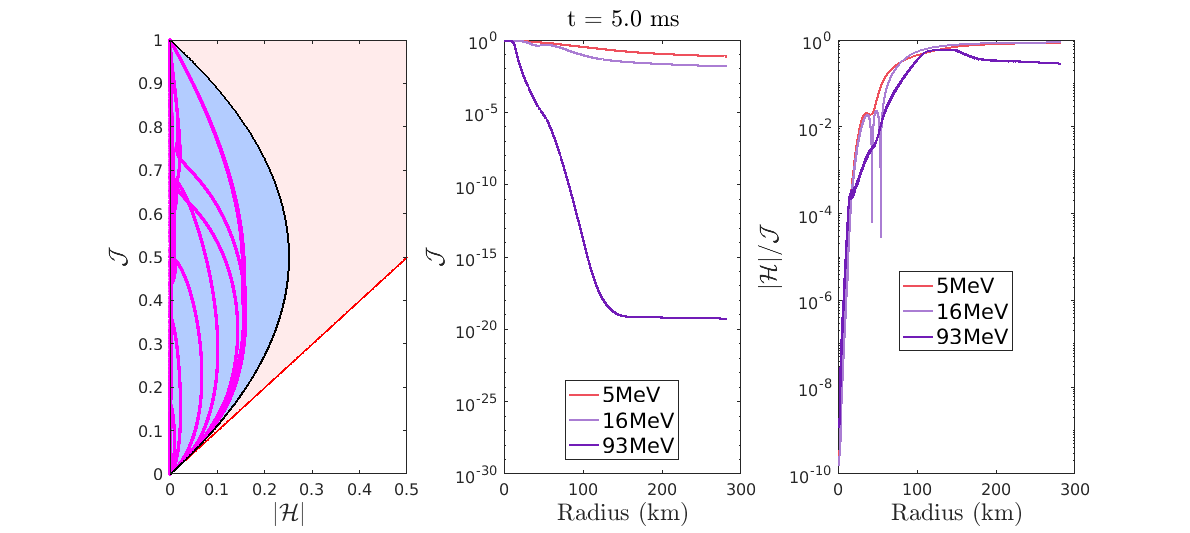
\includegraphics[width=0.45\textwidth]{figures/NSS_5_1}
    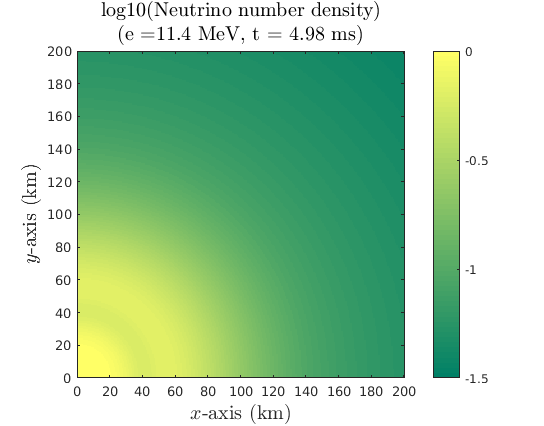
\includegraphics[width=0.45\textwidth]{figures/NSS_5_2} \\
  \end{tabular}
   \caption{Neutrino Stationary State Test}
\end{figure}